%%%%%%%%%%%%%%%%%%%%%%%%%%%%%%%%%%%%%%%%%%%%%%%%%%%%%%%%%%%%%%%%%%%%%%%%%%%%%%%
%%  DR11-South v4 Re-Sweep -- Internal Research Report (sibling to the v3 as-run
%%  campaign report at ../../dr11-campaign/papers/main.tex). Shared tech-report
%%  preamble. Builds with vanilla TeX Live (>= 2022): make pdf
%%  STATUS: SCAFFOLD. Sections 1-3 are drafted from the completed re-sweep;
%%  Sections 4-5 (candidate catalogue + HSC vetting, conclusion) are TODO,
%%  pending the LensJudge v3 cascade vetting of the v4 NEW shortlist.
%%%%%%%%%%%%%%%%%%%%%%%%%%%%%%%%%%%%%%%%%%%%%%%%%%%%%%%%%%%%%%%%%%%%%%%%%%%%%%%
\documentclass[11pt,letterpaper]{article}
\usepackage{../../tech-report}
\usepackage{longtable}
\usepackage{float}

\newcommand{\cnet}{\textsc{ClaudeNet}}
\newcommand{\lj}{\textsc{LensJudge}}
\newcommand{\vb}{\texttt{v3blend8}}
\newcommand{\vc}{\texttt{v4}}

\title{A Release-Native DR11-South Strong-Lens Search:\\
       the \cnet{}~\vc{} Fine-Tuned Re-Sweep}
\author{Greg Benson\thanks{\texttt{benson@cs.usfca.edu}; Department of Computer
        Science, University of San Francisco, CA 94117, USA} \and
        Xiaosheng Huang\thanks{Department of Physics \& Astronomy, University of
        San Francisco; and Physics Division, Lawrence Berkeley National Laboratory}}
\date{June 2026}

\begin{document}
\maketitle
\subtitle{Internal Research Report}

\begin{abstract}
This report is the \cnet{}~\vc{} follow-on to the as-run DR11-south campaign (the sibling report, which
swept and vetted with \vb{} against HSC PDR3 \citep{aihara2022hscpdr3} and SuGOHI
\citep{sonnenfeld2018sugohi}). It documents two release-portable levers and the candidate catalogue they
produce. \textbf{(i)} The apparent DR9$\to$DR11 grade-A recall collapse ($62\%\!\to\!41\%$ at the
$10^{-4}$ operating point) is an \emph{operating-point} artifact, not a model failure: the five-member
calibrated \emph{mean} separates DR11 lenses from random DR11 galaxies at AUC $0.9955$, and replacing the
per-member union with the mean recovers grade-A recall to $75\%$ at the same survivor budget.
\textbf{(ii)} A \emph{release-native warm-start fine-tune} of the three swappable members --- on a
$\sim$13$\times$-expanded native positive pool ($3{,}171$ net-new confirmed lenses) plus DR11-native hard
negatives --- passes a held-out gate, lifting Storfer grade-A recall $0.544\!\to\!0.796$ (the
lrg$+$companion hard residual the resolution-limited \vb{} could not crack). Re-sweeping all
$5.38\times10^{7}$ DR11-south galaxies with the fine-tuned \vc{} ensemble and selecting the top $150$k by
mean yields the \vc{} candidate set, whose held-out recall (Storfer/Inchausti, training-excluded) reaches
\textbf{0.87} (Inchausti grade-A) and \textbf{0.825} (Storfer grade-A) --- the best of any configuration,
and a substantially new pool ($+134$k candidates beyond the union-$95$k). The \vc{} catalogue is
recall-richer but its new candidates are \emph{pending} \lj{} HSC tier-2 vetting (\S\ref{sec:vet}, in
progress); the completed, HSC-vetted catalogue remains the \vb{} as-run set of the sibling report.
\end{abstract}

\section{Premise: a release-native re-sweep}
\label{sec:premise}
The as-run DR11-south campaign (sibling report) established the resolution-limited thesis with \vb{}: a
DESI pre-screen, HSC tier-2 confirmation in the overlap, $24$ HSC-graded A/B (mostly SuGOHI
cross-matches), and an honest ``no net-new lens from DECaLS alone.'' It also surfaced --- but did not
deploy --- the diagnosis that the DR11 recall loss is a stage-1 \emph{selection} artifact. This report
takes the data/calibration lever to its DR11 limit and reports the resulting \vc{} candidate set. Two
levers, both release-portable (the recipe is what transfers to higher-resolution surveys):
\begin{itemize}
  \item a calibrated-\emph{mean} stage-1 selector that removes the DR9$\to$DR11 threshold drift at no
  cost (\S\ref{sec:ensemble});
  \item a release-native warm-start fine-tune of the three swappable members on a re-harvested,
  DR11-native training pool (\S\ref{sec:ensemble}), gated on held-out recall.
\end{itemize}
Both \emph{stack} on \vb{}'s contaminant-aware members; \vc{} keeps the two frozen anchors
(\texttt{effnet\_B}, \texttt{zoobot\_N}) and swaps the three fine-tuned members.

\section{The \vc{} ensemble: mean selection + release-native fine-tune}
\label{sec:ensemble}
\paragraph{Mean combiner.} The stage-1 union over per-member $10^{-4}$ thresholds degrades on the deeper
DR11 imaging (thresholds tighten, the \texttt{resnet46\_C} member saturates), so the union is dominated
by single-member spikes. The calibrated five-member mean instead separates in-parent held-out grade-A
lenses from a $2$M random DR11 negative sample at AUC $0.9955$, recovering grade-A recall $54\%\!\to\!75\%$
at the same $95$k budget and reaching DR10's in-domain $62\%$ at $<\!43$k survivors (Fig.~\ref{fig:recall}).
The mean is adopted as the default stage-1 selector and carries no per-release threshold recalibration.

\begin{figure}[t]\centering
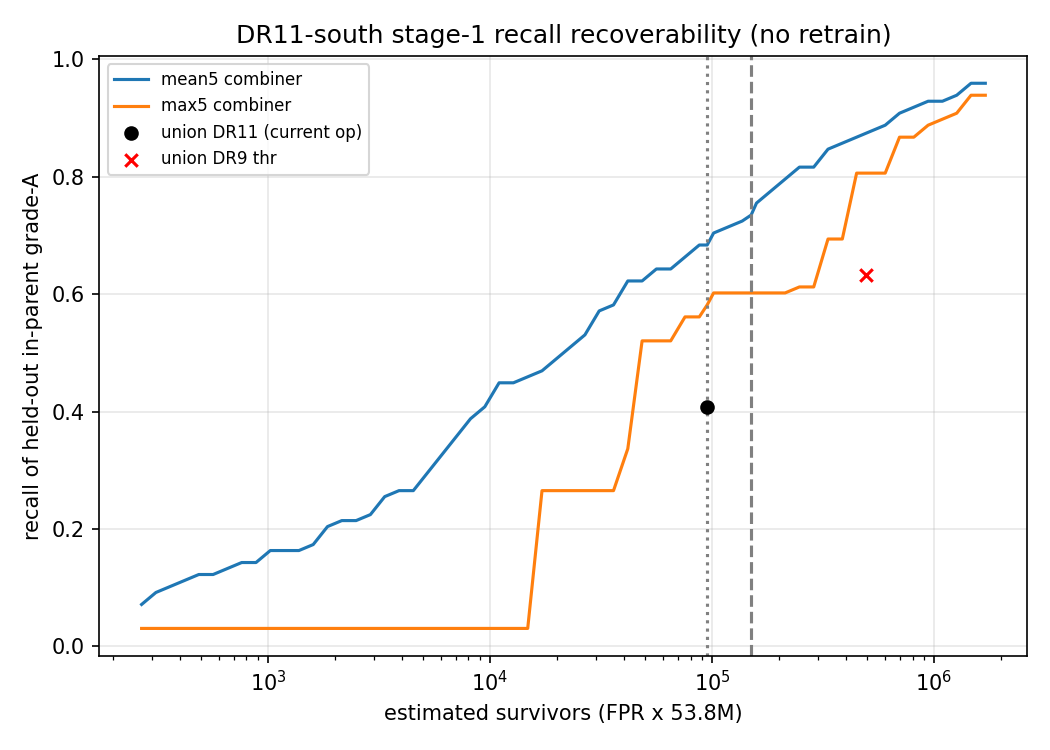
\includegraphics[width=0.72\linewidth]{figures/recall_recoverability.png}
\caption{Held-out grade-A recall vs.\ survivor budget for the mean/max combiners; the per-member union
operating point (black) sits far below the mean at the same budget. The recall loss was the selector,
not the model.}
\label{fig:recall}
\end{figure}

\paragraph{Release-native training pool + fine-tune.} The v1--v3 positive set was capped at $1{,}961$
DR9-pixel lenses. A broad re-harvest of the confirmed-lens literature for the DR11-south footprint
(reclaimed VizieR/DES/KiDS \citep{rezaei2025kids}/HSC catalogs, SLACS/BELLS, lensed-quasar compilations,
a bulk SIMBAD pull, Euclid-Q1 A/B \citep{euclidq1}), deduplicated at $5''$ and tiered by confidence,
yields $3{,}171$ net-new high-confidence positives. All cutouts are re-extracted DR11-native
(\texttt{griz}, $101$\,px), tier-subsampled to $5{,}806$ positives, and paired with $30$k random $+$
$20$k hard DR11 negatives; the three swappable members are warm-started from their \texttt{\_b50}
checkpoints and fine-tuned ($12$ epochs, $\mathrm{lr}{=}3\times10^{-4}$). Storfer and Inchausti
\citep{storfer2024,inchausti2025} are held out (excluded as positives \emph{and} negatives), so the gate
measures generalisation. The fine-tune passes decisively, with the largest gain
on the hard residual (Table~\ref{tab:gate}).

\begin{table}[t]\centering
\caption{\vc{} fine-tune gate: held-out (training-excluded) recall at the matched-FPR $95$k operating
point (calibrated-mean combiner). Baseline is the v3 five-lean ensemble.}
\label{tab:gate}
\begin{tabular}{lccc}
\toprule
held-out set & v3 baseline & \vc{} fine-tuned & $\Delta$ \\
\midrule
Inchausti grade-A & 0.724 & \textbf{0.816} & $+0.09$ \\
Inchausti grade-B & 0.515 & \textbf{0.812} & $+0.30$ \\
Storfer grade-A (hard) & 0.544 & \textbf{0.796} & $+0.25$ \\
\bottomrule
\end{tabular}
\end{table}

\section{The full DR11-south re-sweep and the \vc{} candidate set}
\label{sec:resweep}
We re-scored all $5.38\times10^{7}$ DR11-south galaxies with the fine-tuned \vc{} ensemble --- reusing the
original parent cutouts (no re-extraction), combining the mean of [\texttt{effnet\_B}, \texttt{zoobot\_N},
the three fine-tuned members] --- and selected the top $150$k by mean. Held-out recall climbs monotonically
across the three configurations (Table~\ref{tab:recall}), with the v4 full re-sweep best on every set and
largest on the hard residual. The \vc{} top-$150$k retains only $15{,}922$ of the union-$95$k survivors and
adds $134{,}078$ --- a substantially new, recall-richer candidate pool, the input to the vetting below.

\begin{table}[t]\centering
\caption{Held-out grade-A recall (position-crossmatch; Storfer/Inchausti training-excluded) across the
three DR11-south configurations: the original per-member union operating point, the mean re-rank of the
old five-lean ensemble, and the full \vc{} re-sweep.}
\label{tab:recall}
\begin{tabular}{lccc}
\toprule
held-out set & union-$95$k & mean-$150$k (v3-lean) & \textbf{\vc{} re-sweep} \\
\midrule
Inchausti grade-A & 0.54 & 0.80 & \textbf{0.87} ($60/69$) \\
Inchausti grade-B & --- & --- & \textbf{0.87} ($76/87$) \\
Storfer grade-A (hard) & 0.32 & 0.61 & \textbf{0.825} ($85/103$) \\
\bottomrule
\end{tabular}
\end{table}

\section{Candidate catalogue and \lj{}~v3 HSC vetting}
\label{sec:vet}
% TODO (pending the LensJudge v3 cascade vetting of the v4 NEW shortlist):
%  - the v4 NEW (not-in-any-catalog) shortlist drawn from survivors_dr11s_v4.parquet (394-style
%    re-rank + crossmatch), top-N by the v4 mean;
%  - the LensJudge v3 cascade (DESI tier-1 -> HSC PDR3 tier-2) vetting results on that shortlist:
%    HSC-graded A/B count, SuGOHI cross-validation, genuinely-new systems;
%    direct A/B comparison vs the v3 as-run vetted set (sibling report);
%  - residual-robustness / honest-grader caveats carried over;
%  - per-candidate gallery (appendix).
\emph{In progress.} The \vc{} candidate set (top-$150$k by mean; the NEW, not-in-any-catalog shortlist
extracted as in the sibling report) is queued for the \lj{}~v3 cascade (DESI tier-1 triage $\to$ HSC PDR3
tier-2 escalation). This section will report the HSC-graded A/B yield, the SuGOHI cross-validation, the
genuinely-new systems, and the A/B comparison against the \vb{} as-run vetted catalogue. Until then the
\emph{confirmed} DR11-south catalogue is the \vb{} as-run set of the sibling report; the \vc{} set here is
the recall-richer candidate pool from which the next vetting pass draws.

\section{Conclusion}
\label{sec:conclusion}
% TODO: finalise once vetting (Sec. 4) completes.
\emph{Pending vetting (\S\ref{sec:vet}).} Provisionally: the \vc{} levers --- mean selection and a
release-native warm-start fine-tune --- recover and exceed in-domain DR11-south recall and, for the first
time, crack the lrg$+$companion hard residual, yielding a recall-richer candidate set at the unchanged
DECaLS resolution ceiling. Whether this converts to \emph{net-new} confirmed lenses is the question the
HSC tier-2 vetting (\S\ref{sec:vet}) will answer; the resolution lever (HSC/Euclid) remains decisive.

\bibliographystyle{plainnat}
\bibliography{references}
\end{document}
